%version of 07-03-19

\chapter{SETS AND THEIR ALGEBRAS: \\
The Stem Cells of Mathematics}
\label{ch:sets-BA-logic}


%\begin{quote}
%{\em Sets are the stem cells of mathematics, hence also of science}
%\end{quote}

\section{Introduction}

This chapter studies three of the most basic concepts that underlie
mathematics:
\begin{enumerate}
\item
Sets: ``pure'' objects, with no structure or apparent capability of
operating on anything nor being operated on
\item
Structured sets: sets whose objects have structure connoting their
relationships with other objects
\item
Algebras: sets, with or without structure, enriched by operations that
operate either on the sets or on their objects.
\end{enumerate}
We describe these concepts informally in this introductory section.


\bigskip

{\it Basic sets.} \index{set} (Section~\ref{sec:sets}) Sets are
probably the most basic object of mathematical discourse.  Sets exist
to have {\it elements}, \index{set!element} or {\it members},
\index{set!member} the entities that {\em belong to} 
\index{set!the belong-to relation} the set.  Despite the conceptual
simplicity of the notion ``{\it set}'', that notion is surprisingly
difficult to specify formally; philosophers have been debating the
nature of the notion for millennia.  Yet, the intuitive grasp of the
concept that {\em everyone} develops just in the course of living is
surprisingly adequate for almost all intellectual endeavors regarding
the concept---so, we take the basic definition of ``set'' as given,
and we begin our joint journey into the wondrous world of mathematics
from that point.  We begin to develop the rudiments of science and
mathematics by imposing structure upon the sets of interest and
assembling a repertoire of operations to manipulate them.

As soon as our mathematical progenitors began to develop a repertoire
of operations on sets, they began to observe patterns regarding how
various operations interact with one another.  As understanding of the
operations increased, many of the patterns evolves into the {\em
  ``laws''} that govern interactions among the operations.  Two
familiar ``laws'' assert that one can add a set of numbers in a
variety of ways without affecting the sum:
\begin{itemize}
\item
{\it The commutative law.}
\[ (\forall x_1, x_2) \ \big[ x_1 + x_2 \ = \ x_2 + x_1 \big] \]

\item
{\it The associative law.}
\[ (\forall x_1, x_2, x_3) \ \big[ \big(x_1 + (x_2 + x_3)\big) \ \
= \ \ \big((x_1 + x_2) + x_3\big) \big]
\]
\end{itemize}

\bigskip

\noindent \fbox{
\begin{minipage}{0.95\textwidth}
\underline{\it Laws: in society, in science, in mathematics}

Unfortunately, the word ``law'' plays at least three mutually
inconsistent roles in our lives.
\index{laws: in society, in science, in mathematics}
\begin{enumerate}
\item
We read one day in a newspaper about a new ``law'' that has been
enacted by governmental entities.  The next day, we read about a
``law''---perhaps the one that was just enacted---that has been
amended or even abrogated.  These ``laws'' have finite lifetimes which
are at the whim of governmental entities.

\item
We learn in school about certain ``laws'' of physics---the ``law'' of
gravity, the ``law'' of relativity, the ``law'' of conservation of
mass, to name just a few.  As time goes by and new science is
discovered, some of these ``laws'' get amended---we learn, for
instance, that mass and energy are not conserved: they are, in fact,
interchangeable.  Indeed, some ``laws'' are discovered to have been
{\em false}---the tale of {\it phlogiston} comes to mind.  These
``laws'' are {\em approximations to reality} that will survive until
``laws'' are discovered that are better approximations.

\item
We either learn about or discover certain mathematical facts that
become known as {\em ``laws''}.  We discover, for instance, that one
can add a list of numbers in any order without changing the sum.
These ``laws'' are immutable.  They are not based on human experience
to any point in time but rather on logical reasoning about specific
constants of life: numbers, geometrical shapes, etc.  These are the
``laws'' that we will begin to uncover in this and subsequent chapters.
\end{enumerate}
\end{minipage}
}
\bigskip

\noindent
Having clarified our intent, we shall no longer place the word ``law''
in quotes.

\bigskip

{\it Structured sets}. \index{set!structured}
(Section~\ref{sec:structured-set}) The first operations on sets that
we study endow sets with enough structure to talk about ``real life''.
One can view these operations as the mathematical analogue of
``systems programs'' within the realm of computers.
\begin{itemize}
\item
We formulate a rigorous analogue of the intuitive concept of {\it
  relation}.  We can thenceforth talk about relations such as
``parent-child'', ``set-subset'', ``numbers and their squares'', and
we can study how some of these relations behave like---or
unlike---some others.
\item
We use various kinds of structure in sets to create complex objects
that have sub-objects and sub-$\cdots$-objects to arbitrary depths.
\item
We identify the notion {\it function}, which is among the central
concepts of mathematics, and we identify valuable genres of function
(one-to-one, onto, \ldots).
\end{itemize}
Once we have these notions, we can begin to formulate realistic {\it
  mathematical models} for real-life entities.  Two features that will
stand out: how naturally the formal notions capture the intuitive
notions of the vernacular; how technically simple the formal notions
are---which facilitates using them in sophisticated analyses.

\bigskip

{\it Algebras}.  (Section~\ref{sec:Boolean-Algebra})
\index{algebra}\index{algebra!of sets} Once one has a set, plus
operations on the set which obey laws, one has an {\it algebra}.
\index{algebra!definition} There are several natural algebras whose
objects are sets.  We shall discuss two of them at some length.
\begin{itemize}
\item
{\it Boolean algebras}.  We focus first on the algebra that is built
upon sets and the most basic operations on sets: {\it union} and {\it
  set difference}.  The first of these, denoted $S \cup T$, combines
the membership of its argument sets, $S$ and $T$; the second, denoted
$S \setminus T$, excludes from set $S$ all members of set $T$.  These
two operations provide a basis for the algebra of sets, in the sense
that one can combine these two operations in myriad ways to craft an
immense repertoire of operations on sets.  As an exercise, the reader
should define the following two operations from union and set
difference: {\it intersection} ($S \cap T$), which isolates all
elements that sets $S$ and $T$ share, and {\it symmetric difference}
($S+T$), which isolates all elements that belong to precisely one of
$S$ and $T$.

Importantly, we can now begin to study the laws that these operations
obey.  One of the central topics in this study is the class of {\it
  Boolean} algebras \index{algebra!Boolean algebras} whose name
derives from that of the British mathematician George
Boole. \index{Boole, George}

\item
{\it Propositional Logic}. \index{logic} \index{logic!propositional}
It is difficult to explain the meaning of the Boolean set operations
without using ``logical'' terms such as {\it and}, {\it or}, and {\it
  not}.  These terms fall naturally within the domain of the simplest
variety of {\it mathematical logic}---the {\it logic of propositions},
or, more familiarly, {\it Propositional Logic}.  This branch of logic
studies how the {\em truth-values}, {\sc true} and {\sc false}, of
elementary logical expressions combine via operators such as {\sc
  and}, {\sc or}, and {\sc not} to produce a truth-value for any
complex logical expression.

Propositional Logic is the simplest form of mathematical logic because
it does not deal with the subtleties that arise from issues such as:
{\it quantifiers}---such as ``{\sc there exists}'' ($\exists$), or
``{\sc for all}'' ($\forall$)---or {\it modalities}---such as ``{\sc
  eventually}'' or ``{\sc from some moment on}''.

Propositional Logic is a fascinating special form of Boolean algebra
for at least two reasons.
  \begin{itemize}
  \item
Propositional Logic enjoys a special algebraic feature known as {\it
  free-ness}, which enables one to prove theorems in Propositional
Logic using {\em truth tables:} this amounts to proving theorems
within this system by symbolic evaluation rather than via the axioms
plus rules of inference that we all found so onerous in high school
geometry.
  \item
There is a genre of Propositional logical expression that, by modeling
a genre of {\em computation} faithfully, can serve as a foundation for
a theory of computational complexity.
  \end{itemize}
\end{itemize}


\medskip

This will be an exciting chapter to start our study of mathematics with.

\section{Sets}
\label{sec:sets}

\subsection{Fundamental Set-Related Concepts}
\label{sec:set-concepts}

The reader certainly knows informally what a set is and recognizes
that some sets are finite, while others are infinite.  Continuing to
speak informally---a formal treatment will follow in later
chapters---here are a few illustrative finite sets:
\begin{itemize}
\item
the set of words in this book

We do not know how big this set is, but you as a reader likely have a
better idea than we as authors.
\item
the set of characters in any {\it JAVA} program

Note that while this set is surely finite, we are not so confident
about the number of seconds that a given program will run!
\item
the set consisting of {\em you}

Paraphrasing the iconic television figure Mister Rogers, ``You are
unique.''  This set has just one element.

\item
the set of unicorns in New York City

We will not argue with you about this, but we suspect that this is the
{\em empty set} $\emptyset$, which has zero members.
\end{itemize}
Some familiar infinite sets are:
\begin{itemize}
\item
the set of {\em nonnegative integers}
\item
the set of {\em positive integers}
\item
the set of {\em all integers}
\item
the set of nonnegative {\em rational numbers}---which are quotients of
integers
\item
the set of nonnegative {\em real numbers}---which can be viewed
computationally as the set of numbers that admit infinite decimal
expansions,
\item
the set of {\em complex numbers}---which can be viewed as ordered
pairs of real numbers,
\item
the set of {\em all} finite-length binary strings.

A {\it binary string}\index{binary string} is a sequence of $0$s and
$1$s.  When discussing computer-related matters, one often calls each
$0$ and $1$ that occurs in a binary string a {\it bit}
\index{bit: binary digit} (for {\it binary digit}).  The term ``bit''
leads to the term {\it bit string} \index{bit string} as a synonym of
{\it binary string}.
\end{itemize}
Despite this assumption, we begin the chapter by reviewing some basic
concepts concerning sets and operations thereon.

As noted early, sets were created to contain members/elements.  We
denote the fact that element $t$ {\it belongs to},
\index{set!the belongs-to relation} or, {\it is an element of} set $T$
by the notation $t \in T$.\index{set!membership: $\in$}  Contrarily,
we denote the fact that element $t$ {\it does not belong to},
\index{set!the belongs-to relation} or, {\it is not an element of} set
$T$ by the notation $t \not\in T$.\index{set!membership: $\not\in$} 

A {\em subset}\index{set!subset} of a set $T$ is a set $S$ each of
whose members belongs to $T$.  The subset relation occurs in two
forms, The {\em strong} form of the relation, denoted $S \subset
T$,\index{set!strong subset relation} says that every element of $S$
is an element of $T$, but {\em not} conversely; i.e., $T$ contains
(one or more) elements that $S$ does not.  The {\em weak} form of the
relation, denoted $S \subseteq T$,\index{set!weak subset relation} is
defined as follows:
\[
[S \subseteq T] \ \ \mbox{ means: } \ \
\Big[ \mbox{\em either } \ \ [S = T]
\ \ \mbox{\em or } \ \ [S \subset T] \Big].
\]

For any finite set $S$, we denote by $|S|$ the {\it cardinality}
\index{set!cardinality}\index{cardinality!finite set} of $S$, which is
the number of elements in $S$.  Finite sets having three special
cardinalities are singled out with special names.  The limiting case
of finite sets is the {\em empty set}; this set, which we denote by
$\emptyset$ is {\em unique}.  We say that, $\emptyset$ is {\it
  characterized} by the equation $|\emptyset| = 0$, meaning that the
equation can be used as a definition of the set.  (The empty set is
often a limiting case of set-defined entities.)  If $|S| = 1$, then we
call $S$ a {\em singleton};\index{set!singleton set} and if $|S| = 2$,
then we call $S$ a {\em doubleton}.\index{set!doubleton} (One could,
of course, continue with ``tripletons'' and ``quadrupletons'', etc.,
but people tend not to do this.)

It is often useful to have a convenient term and notation for {\em the
  set of all subsets of a set $S$}.  This bigger set---we shall see
that it contains $2^{|S|}$ elements when $S$ is finite---is denoted
$\p(S)$ and is called the {\em power set}
\index{power set:set of all subsets} of $S$.\footnote{The name ``power
  set'' arises from the relative cardinalities of $S$ and ${\cal
    P}(S)$ for finite $S$.}  Note carefully the two set-relations that
we are talking about here: 

\hspace*{.35in}{\em If set $T$ is a {\em subset} of set $S$, then $T$
  is an {\em element} of the set $\p(S)$.}

\noindent
You should satisfy yourself that the biggest and smallest elements of
${\cal P}(S)$ are, respectively, the set $S$ itself and the empty set
$\emptyset$.

\subsection{Operations on Sets}
\label{sec:set-operations}

Given two sets $S$ and $T$ depicted in Fig.~\ref{fig:setInitial}, we denote by:
\begin{figure}[htb]
\begin{center}
        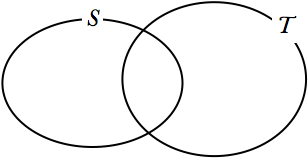
\includegraphics[scale=0.4]{FiguresMaths/setInitial}
        \caption{Two sets $S$ and $T$.}
        \label{fig:setInitial}
\end{center}
\end{figure}
\begin{itemize}
\item
$S \cap T$\index{$S \cap T$: set intersection} the {\it
  intersection}\index{set!operations!intersection}
of $S$ and $T$: the set of elements that belong to {\em both} $S$ and
$T$ (see Fig.~\ref{fig:setIntersection}).
\[ [s \in S \cap T] \ \ \mbox{ means } \ \ 
\Big[ [s \in S] \ \mbox{\bf and } \ [s \in T] \Big]
\]
\begin{figure}[htb]
\begin{center}
        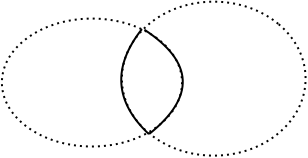
\includegraphics[scale=0.4]{FiguresMaths/setIntersection}
        \caption{Intersection of $S$ and $T$ {\Denis presents also the symmetric difference}.}
        \label{fig:setIntersection}
\end{center}
\end{figure}
\item
$S \cup T$\index{$S \cup T$: set union} the {\it
  union}\index{set!operations!union}
of $S$ and $T$: the set of elements that belong to $S$, or to $T$, {\em
  or to both}.  (Because of the ``or both'' qualifier, this operation
is sometimes called {\em inclusive
  union}.)\index{set!operations!inclusive union}
  Fig.~\ref{fig:setUnion} is an illustration of the union of the sets of Fig.~\ref{fig:setInitial}
\[ [s \in S \cup T] \ \ \mbox{ means } \ \
\Big[ [s \in S] \ \mbox{\bf or } \ [s \in T]  \ \mbox{\bf or } \ [s
    \in S \cap T] \Big]
\]
\begin{figure}[htb]
\begin{center}
        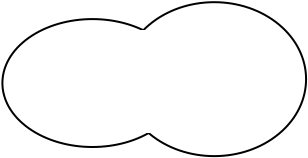
\includegraphics[scale=0.4]{FiguresMaths/setUnion}
        \caption{Union of sets $S$ and $T$.}
        \label{fig:setUnion}
\end{center}
\end{figure}
\item
$S \setminus T$\index{$S \setminus T$: set difference} is the {\em
  (set) difference}\index{set!operations!set difference} of $S$ and
  $T$: the set of elements that belong to $S$ but not to $T$.
\[ [s \in S \setminus T] \ \ \mbox{ means } \ \
\Big[ [s \in S] \ \mbox{\bf and } \ [s \not\in T] \Big]
\]
\begin{figure}[htb]
\begin{center}
        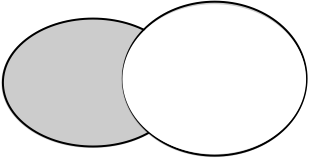
\includegraphics[scale=0.4]{FiguresMaths/setDiff}
        \caption{Difference of sets $S$ and $T$ (in grey).}
        \label{fig:setDiff}
\end{center}
\end{figure}
(Particularly in the United States, one often encounters the notation
 ``$S-T$''\index{$S - T$: set difference} instead of ``$S \setminus
 T$.'')
\end{itemize}

We illustrate the preceding operations with the sets $S = \{a,b,c\}$
and $T = \{c,d\}$.  For these sets:
\begin{eqnarray*}
S \cap T & = &  \{c\}, \\
S \cup T & = & \{a,b,c,d\}, \\
S \setminus T & = & \{a,b\}.
\end{eqnarray*}

In many situations where sets are being studied, the sets of interest
will be subsets of some fixed ``universal'' set
$U$.\index{set!universal set}

\bigskip

\noindent \fbox{
\begin{minipage}{0.95\textwidth}
We use the term ``universal'' contextually, in the sense of a
``universe of discourse''.  We are {\em not} using the term in the
absolute, self-referencing, sense of a set $S$ that contains all sets
as members (``self-referencing'' because set $S$ perforce contains
itself as a member).  The absolute, self-referencing, construct has
been shown by philosopher/logician Bertrand Russell,
\index{Russell, Bertrand} to lead to mind-bending
paradoxes---especially, the eponymous {\it Russell's Paradox}
\cite{Russell02,Russell03}.
\end{minipage}
}
\bigskip

\noindent
Given a universal set $U$ and a {\em subset} $S \subseteq U$,
we observe the set-inequalities
\[ \emptyset \ \subseteq \ S \ \subseteq \ U. \]
When studying a context within which there exists a universal set $U$,
we include within our repertoire of set-related operations also the
operation of {\it complementation}
\index{set!operations!complementation}
\begin{itemize}
\item
$\overline{S} \ \eqdef \ U \setminus S$,\index{$\overline{S}$: the
  complement of set $S$ relative to a universal set}
the {\em complement} of $S$ (relative to the universal set $U$).

For instance, the set of odd positive integers is the complement of
the set of even positive integers, relative to the set of all positive
integers.
\begin{figure}[htb]
\begin{center}
        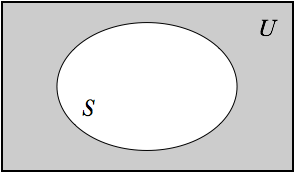
\includegraphics[scale=0.4]{FiguresMaths/setComplement}
        \caption{Complement of set $S$ (in grey) relative to the universal set $U$.}
        \label{fig:setComplement}
\end{center}
\end{figure}
\end{itemize}
We note a number of basic identities involving sets and operations on
them.
\begin{itemize}
\item
$S \setminus T \ = \ S \cap \overline{T}$,
\item
If $S \subseteq T$, then
  \begin{enumerate}
  \item
$S \setminus T \ = \ \emptyset$,
  \item
$S \cap T \ = \ S$,
  \item
$S \cup T \ = \ T$.
  \end{enumerate}
\end{itemize}
Note, in particular, that\footnote{``iff'' is the common abbreviation
  for the mathematical phrase, ``if and only if.''}
\[ [S = T] \ \mbox{  iff  } \ \ \Bigl[[S \subseteq T] \mbox{
    {\small\sf and} } [T \subseteq S]\Bigr] \ \mbox{  iff  }
\ \ \Bigl[ (S \setminus T) \cup (T \setminus S) = \emptyset\Bigr].
\]

The operations union, intersection, and complementation---and
operations formed from them, such as set difference---are usually
called the {\em Boolean (set) operations},\index{Boolean set operations}
\index{set!operations!Boolean set operations} so named for the
$19$th-century English mathematician George Boole.
\index{Boole, George} There are several important identities involving
the Boolean set operations.  Among the most frequently invoked are the
two {\em laws} attributed to the $19$th-century French mathematician
Auguste De Morgan: \index{set!operations!De Morgan's Laws}
\index{De Morgan's Laws}
\begin{equation}
\label{e.de-morgan}
\mbox{For all sets $S$ and $T$: } \ \left\{
\begin{array}{lcl}
\overline{S \cup T} & = & \overline{S} \cap \overline{T}, \\
 \\
\overline{S \cap T} & = & \overline{S} \cup \overline{T}.
\end{array}
\right.
\end{equation}
Elementary logic can be used to verify these laws.  To spell out just
one case: An element $s$ that belongs to neither $S$ nor $T$ ($s \in
\left(\overline{S} \cap \overline{T}\right)$) cannot belong to the
union of $S$ and $T$.

\medskip

\noindent {\em (Algebraic) Closure}.\index{(Algebraic) Closure}
%
We end this section with a set-theoretic definition that one
encounters in many contexts.  Let $\cal C$ be any (finite or infinite)
collection of sets, and let $S$ and $T$ be two elements of $\cal C$.
{\em (Note that $\cal C$ is a set whose elements are sets.)}  Think,
e.g., of the concrete example of set intersection.

We say that $\cal C$ is {\em closed} under intersection if whenever
sets $S$ and $T$ (which could be the same set) both belong to $\cal
C$, the set $S \cap T$ also belongs to $\cal C$.  By De Morgan's laws,
$\cal C$'s closure under union implies also its closure under
intersection.

\section{Structured Sets}
\label{sec:structured-set}
\index{set!structured}

The power of set-theoretic concepts to model complex aspects of
reality increases immeasurably when we consider sets whose elements
enjoy even modest structure.  We begin our discussion of structured
sets by adding a new (binary) set operation to our earlier repertoire.

Given (finite or infinite) sets $S$ and $T$ we denote by $S \times T$
\index{$S \times T$} the {\it direct product} of $S$ and $T$,
\index{direct product of sets} which is the set of all {\it ordered
  pairs} \index{ordered pair of set elements} whose first coordinate
contains an element of set $S$ and whose second coordinate contains an
element of set $T$.  The direct product operation is often called the
{\it Cartesian} product, \index{Cartesian product of sets} because of
the notion's origin in the formulation of Analytical Geometry by the
French mathematician-philosopher Ren\'{e} Descartes. 
\index{Descartes, Ren\'{e}!inventor of Analytical Geometry}

We illustrate the direct product in two ways, in order to capture all
of its subtleties: Textually, if $S = \{a,b,c\}$ and $T = \{c,d\}$,
then
\[ S \times T \ =  \{
\langle a,c \rangle,
\langle b,c \rangle,
\langle c,c \rangle,
\langle a,d \rangle,
\langle b,d \rangle,
\langle c,d \rangle\}
\]
Pictorially,
Fig.~\ref{fig:cartesianproduct} provides a general illustration of
the direct product $A \times B$ of sets $A$ and $B$.
\begin{figure}[htb]
\begin{center}
        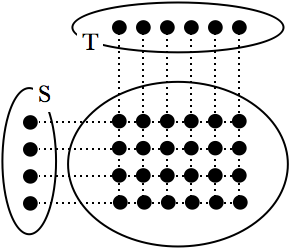
\includegraphics[scale=0.4]{FiguresMaths/cartesianProduct}
        \caption{The Direct product of sets $A$ and $B$.}
        \label{fig:cartesianproduct}
\end{center}
\end{figure}

\subsection{Binary Relations: Sets of Ordered Pairs}
\label{sec:relation}

The direct-product operation on sets affords us a simple, yet
powerful, formal notion of binary relation.  Given (finite or
infinite) sets $S$ and $T$, a {\it relation $\rho$ on $S$ and
  $T$}\index{relation on sets} (in that order) is any subset
\[ \rho \ \subseteq \ S \times T. \]
When $S = T$, we often call $\rho$ a {\em binary relation on (the set)
  $S$}\index{binary relation on a set} (``{\em binary}'' because there
are {\em two} copies of set $S$ being related by $\rho$).

Relations are so common that we use them in every aspect of our lives
without even noticing them.  The relations ``equal to,'' ``less
than,'' and ``greater than or equal to'' are simple examples of binary
relations on the integers.  These same three relations apply also to
other familiar number systems such as the rational and real numbers;
only ``equal,'' though, holds (in the natural way) for the complex
numbers. (You will see much more about these sets of numbers in coming
chapters.)  Some subset of the three relations, ``is a parent of,''
``is a child of,'' and ``is a sibling of'', are binary relations that
may apply to (the set of people constituting) your family.  The
preceding relations all apply to a single set $S$; a familiar relation
for which the sets $S$ and $T$ are distinct is the relation ``$A$ is
taking course $X$''; it is a relation on
\[ \left( \mbox{the set of all students} \right) \times
   \left( \mbox{the set of all courses} \right).
\]

\ignore{************
We shall see later (Section~\ref{s.pairing}) that there is a formal
sense in which binary relations are all we ever need consider: $3$-set
({\em ternary}) 
relations\index{ternary relation}\index{relation!ternary}---which are
subsets of $S_1 \times S_2 \times S_3$---and $4$-set ({\em
  quaternary}) 
relations\index{quaternary relation}\index{relation!quaternary}---which
are subsets of $S_1 \times S_2 \times S_3 \times S_4$---and so on (for
any finite ``arity''), can all be expressed as binary relations of
binary relations \ldots of binary relations.  As examples: For ternary
relations, we can replace any subset $R$ of $S_1 \times S_2 \times
S_3$ by the obvious corresponding subset $R'$ of $S_1 \times (S_2
\times S_3)$: for each element $\langle s_1, s_2, s_3 \rangle$ of $R$,
the corresponding element of $R'$ is $\langle s_1, \langle s_2, s_3
\rangle \rangle$.  Similarly, for quaternary relations, we can replace
any subset $R''$ of $S_1 \times S_2 \times S_3 \times S_4$ by the
obvious corresponding subset $R'''$ of $S_1 \times (S_2 \times (S_3
\times S_4))$: for each element $\langle s_1, s_2, s_3, s_4 \rangle$
of $R''$, the corresponding element of $R'''$ is $\langle s_1, \langle
s_2, \langle s_3, s_4 \rangle \rangle \rangle$.
\begin{quote}
You should convince yourself that we could achieve the desired
correspondence also by replacing $S_1 \times (S_2 \times S_3)$ with
$(S_1 \times S_2) \times S_3$ and by replacing $S_1 \times S_2 \times
S_3 \times S_4$ by either $((S_1 \times S_2) \times S_3) \times S_4$
or $(S_1 \times S_2) \times (S_3 \times S_4)$.
\end{quote}
************}

By convention, when dealing with a binary relation $\rho \ \subseteq
\ S \times T$, we often write ``$s \rho t$''\index{infix notation for
  a binary relation: $s \rho t$} in place of the more stilted notation
``$\langle s, t \rangle \in \rho$.''  For instance we (almost always)
write ``$5 < 7$'' in place of the strange-looking (but formally
correct) ``$\langle 5,7 \rangle \in \ <$.''

The following operation on relations occurs in many guises, in almost
all mathematical theories.  Let $\rho$ and $\rho'$ be binary relations
on a set $S$.  The {\it composition}
\index{composition! binary relations}\index{composition of binary relations}
of $\rho$ and $\rho'$ (in that order) is the relation
\[ 
\rho'' \ \eqdef \ \Bigl\{ \langle s, t \rangle \in S \times S \ | \
(\exists u \in S) \Bigl[ [s \rho u] \mbox{ and } [u \rho' t] \Bigr] \Bigr\}.
\]
Note that we have used both of our notational conventions for
relations in the preceding equation.  We also encounter here, for the
first time in the text, but certainly not the last, a new notational
convention: the common ``shorthand'' compound symbol ``$\eqdef$'':
\index{$\eqdef$: ``equals, by definition''} The sentence ``$X \eqdef
Y$'' should be read \\
\hspace*{.25in}``$X$ {\em is (or, equals), by definition}, $Y$.''

\bigskip

\noindent \fbox{
\begin{minipage}{0.95\textwidth}
Even at this stage in our study, we encounter concepts that appear
directly in ``real-life'' applications.  The operation of {\em
  composing relations} is an essential feature of {\it relational
  databases;} see, e.g., \cite{Codd70}.  
\end{minipage}
}
\bigskip

\noindent
When we discuss a relation $\rho \subset S \times T$, it is important
to be able to assert that elements $s \in S$ and $t \in T$ are {\em
  not} $\rho$-related,\index{relation negation} i.e., $\langle s, t
\rangle \not\in S \times T$.  Several notations have been developed
for this purpose, as the following table suggests.
\index{$\overline{\rho}$: the negation of relation $\rho$}
\begin{equation}
\label{eq:NOT-rho-notation}
\begin{array}{|c|c|c|c|}
\hline
\mbox{\bf Relation} & \mbox{\bf Notation} & \mbox{\bf Negation} &
\mbox{\bf Standard?} \\
\hline
\hline
\mbox{set membership} & \in & \not\in & \mbox{yes} \\
\hline
\mbox{equality}       & =   & \neq    & \mbox{yes} \\
\hline
\mbox{less than (strong)} & < & \not < \mbox{ or } \geq & \mbox{yes} \\
\hline
\mbox{less than (weak)} & \leq & \not\leq \mbox{ or } > & \mbox{yes} \\
\hline
\mbox{greater than (strong)} & > & \not > \mbox{ or } \leq & \mbox{yes} \\
\hline
\mbox{greater than (weak)} & \geq & \not\geq \mbox{ or } < & \mbox{yes} \\
\hline
\mbox{generic}  & \rho  & \neg\rho \mbox{ or } \overline{\rho} &
\mbox{no} \\
\hline
\end{array}
\end{equation}

\medskip

Several special classes of binary relations are so important that we
must single them out immediately, in the upcoming subsections.


\subsection{Order Relations}
\label{sec:order-relation}

A binary relation $\rho$ on a set $S$ is a {\it partial order
  relation},\index{order relation}
\index{order relation!partial}\index{partial order}\index{order} or,
more briefly, is a {\it partial order} if $\rho$ is
transitive.\index{transitive relation} This means that, for all
elements $s, t, u \in S$,
\begin{equation}
\label{eq:def-transitive}
\mbox{if } \ \ sRt \ \ \ \mbox{ and } \ \ tRu \ \ \ \mbox{ then }
\  \ sRu.
\end{equation}
The qualifier ``partial'' warns us that some pairs of elements of $S$
do not occur in relation $\rho$.  Number-related orders supply an easy
illustration.  Given any two {\em distinct} integers, $m$ and $n$, one
of them must be less than the other: either $m < n$, or $n < m$.  In
contrast, if we consider {\it ordered pairs} of integers, then there
are pairs of pairs that are not related by the ``less than'' relation
in any natural way.  For instance, even though we may agree that (by a
natural extension of the number-ordering relation ``less than'') the
ordered-pair $\langle 4, 17 \rangle$ is ``less than'' the ordered-pair
$\langle 22, 19 \rangle$, we might well not agree on which of the
ordered-pairs $\langle 4, 22 \rangle$ and $\langle 19, 17 \rangle$ is
``less than'' the other.

\ignore{\Arny The distinction between strong and weak orders is important,
  but there is probably a less formalistic way to explain the
  difference.  Please try}

In many domains, order relations occur in two ``flavors'', {\em
  strong} and {\em weak}.\index{order!strong}\index{order!weak} For
many such relations $\rho$---consider, e.g., ``less than'' on the
integers---the weak version is denoted by underscoring the strong
one's symbol.  This will be our convention.  Just as $\leq$ denotes
the weak version of $<$, and $\geq$ denotes the weak version of $>$,
we shall denote the weak version of a generic order $\rho$ by
$\underline{\rho}$.
\index{$\underline{\rho}$:the weak version of order relation $\rho$}
Strong and weak versions of an order relation $\rho$ (denoted,
respectively, $\rho$ and $\underline{\rho}$) are distinguished by
their behavior under simultaneous membership.  For illustration,
instantiate the following template with $\rho$ being ``$<$'' and with
$\rho$ being ``$>$'':

\smallskip

\begin{tabular}{lll}
For a strong order $\rho$: & &
{\bf if} $[s \ \rho \ t]$, {\bf then} $[t \ \overline{\rho} \ s]$ \\
For the weak version $\underline{\rho}$ of $\rho$: & &
{\bf if} $[s \ \underline{\rho} \ t]$ {\bf and} $[t \ \underline{\rho}
  \ s]$, {\bf then} $[s = t]$.
\end{tabular}

\medskip

It is important to note that negating a strong relation (e.g., $<$)
yields a weak relation ($\geq$), while negating a weak relation (e.g.,
$\leq$) yields a strong relation ($>$).  Keep this in mind when we
study Propositional Logic in Section~\ref{sec:Propositional-logic}.
We shall note there that the following transformations
\begin{eqnarray*}
\mbox{weak order} + \mbox{negation} 
 & \longrightarrow & \mbox{strong order} \\
\mbox{strong order} + \mbox{negation}
 & \longrightarrow & \mbox{weak order}
\end{eqnarray*}
result from Proposition~\ref{thm:De-Morgan}, the logical analogue of
De Morgan's Laws (\ref{e.de-morgan}).

\subsection{Equivalence Relations}
\label{sec:equiv-relation}

A binary relation $\rho$ on a set $S$ is an {\it equivalence relation}
\index{equivalence relation} \index{relation!equivalence relation} 
if it enjoys the following three properties:

\medskip

\begin{tabular}{llll}
1. &
$\rho$ is {\em reflexive:}
   & $(\forall s \in S)$ & $[s \rho s]$ \\
2. &
$\rho$ is {\em symmetric:}
   & $(\forall s, s' \in S)$ 
& $\left[ [s \rho s'] \ \mbox{ iff } \ [s' \rho s] \right]$ \\
3. &
$\rho$ is {\em transitive:}
   & $(\forall s, s', s'' \in S)$ & if both \
$[s \rho s'] \ \mbox{ and } \ [s' \rho s''], \ \mbox{ then also } \ [s \rho s'']$
\end{tabular}

\medskip

\noindent
Sample familiar  equivalence relations are:
\begin{itemize}
\item
The equality relation $=$ on a set $S$.

This relation relates each $s \in S$ with itself (i.e., $s=s$) but
with no other element of $S$.

\item
The relations $\equiv_{12}$ and $\equiv_{24}$ on integers,
where\footnote{As usual, $|x|$ is the {\em absolute value}, or, {\em
    magnitude} of the number $x$.  That is, if $x \geq 0$, then $|x| =
  x$; if $x < 0$, then $|x| = -x$.}
  \begin{enumerate}
  \item
$n_1 \equiv_{12} n_2$ if and only if $|n_1 - n_2|$ is divisible by
$12$.
  \item
$n_1 \equiv_{24} n_2$ if and only if $|n_1 - n_2|$ is divisible by
$24$.
  \end{enumerate}
We use relation $\equiv_{12}$ (without formally acknowledging it) when
we tell time using a $12$-hour clock; we use relation $\equiv_{24}$
when we tell time using a $24$-hour clock.
\end{itemize}

\noindent
Closely related to the notion of an equivalence relation on a set $S$
is the notion of a {\it partition} \index{partition}
\index{set!partition} of $S$---i.e., a nonempty collection of subsets
$S_1, S_2, \ldots$ of $S$ that are

\smallskip

\begin{tabular}{l}
{\em mutually exclusive:}
for distinct indices $i$ and $j$, $S_i \cap S_j = \emptyset$; \\
and  \\
{\em collectively exhaustive:}
$S_1 \cup S_2 \cup \cdots = S$.
\end{tabular}

\smallskip

\noindent
We call each set $S_i$ a {\it block} of the partition. \index{partition!block}
\index{set!partition!block} \index{block of a partition}

\noindent
One verifies the following Proposition easily.
\index{partitions!and equivalence relations} 
\index{equivalence relations!and partitions} 

\begin{prop}
A partition of a set $S$ and an equivalence relation on $S$ are just
two ways of looking at the same concept.
\end{prop}

\begin{proof}[Sketch]
{\it To get an equivalence relation from a partition}.
Given any partition $S_1, S_2, \ldots$ of a set $S$, define the
following relation $\rho$ on $S$:

$s \rho s'$ if and only if $s$ and $s'$ belong to the same block of the
partition.

\noindent
We claim that relation $\rho$ is an equivalence relation on $S$.  To
wit, the {\em collective exhaustiveness} of the partition ensures that
each $s \in S$ belongs to some block of the partition, while {\em
  mutual exclusivity} ensures that $s$ belongs to only one block.

\noindent {\it To get a partition from an equivalence relation}.
Focus on any equivalence relation $\rho$ on a set
$S$.  For each $s \in S$, denote by $[s]_\rho$ the set
\[ [s]_\rho \ \eqdef \ \{ s' \in S \ | \ s \rho s' \} \]
we call $[s]_\rho$ {\it the equivalence class of $s$ under relation
$\rho$}.\index{equivalence class}\index{equivalence relation!class}

\noindent
{\em The equivalence classes under $\rho$ form a partition of $S$}.
To wit: $\rho$'s {\em reflexivity} ensures that the equivalence classes
collectively exhaust $S$; $\rho$'s symmetry and transitivity ensure that
equivalence classes are mutually disjoint.  \qed
\end{proof}

The {\it index} \index{index (of an equivalence relation)}
\index{equivalence relation!index} \index{relation!equivalence
  relation!index} of the equivalence relation $\rho$ is its number of
classes---which can be finite or infinite.  Henceforth, we conform to
common usage and use the symbol $\equiv$, possibly embellished by a
subscript or superscript, to denote an equivalence relation.

Let $\equiv_1$ and $\equiv_2$ be two equivalence relations on a set
$S$.  We say that the relation $\equiv_1$ {\em is a refinement of}
(or, {\em refines})\index{refinement of an equivalence relation} 
\index{equivalence relation!refinement}
the relation $\equiv_2$ precisely when each block of $\equiv_1$ is a
subset of some block of $\equiv_2$.  We leave to the reader the simple
verification of the following basic result.


\begin{theorem}
\label{thm:equality=finest-equiv}
The equality relation, $=$, on a set $S$ is the {\em finest}
equivalence relation on $S$, in the sense that $=$ refines every
equivalence relation on $S$.
\end{theorem}

\subsection{Functions}
\label{sec:function}
\index{function}

One learns early in school that a function from a set $A$ to a set $B$
is a rule that assigns a unique value from $B$ to every value from
$A$.  Simple examples illustrate that this notion of function is more
restrictive than necessary.  Think, e.g., of the operation {\em
  division} on integers.  We learn that division, like multiplication,
is a function that assigns a number to a given pair of numbers---yet
we are warned immediately not to ``divide by $0$'': The quotient upon
division by $0$ is ``undefined.''  So, division is not quite a
function of the same sort as addition or multiplication, which both
{\em do} conform to the notion envisioned by our initial definition of
``function''.  In more homely terms, note that, in contrast to an
expression such as ``$4 \div 2$,'' which should lead to the result $2$
in every programming environment,\footnote{We are, of course, ignoring
  demons such as round-off error.}~expressions such as ``$4 \div 0$''
can lead to wildly different results in different programming
environments.  Since ``wildly different'' is anathema in any
mathematical setting, mathematicians have dealt with situations such
as one encouters with division by broadening the definition of
``function'' in a way that behaves like our initial simple definition
under ``well-behaved'' circumstances and that extends the notion in an
intellectually consistent way under ``ill-behaved'' circumstances.
Let us begin to get formal.

A {\it (partial) function from set $S$ to set $T$} is a relation $F
\subseteq S \times T$ that is {\it single-valued;} i.e., for each $s
\in S$, there is {\em at most} one $t \in T$ such that $sFt$.  We
traditionally write ``$F: S \rightarrow T$'' as shorthand for the
assertion, ``$F$ is a function from the set $S$ to the set $T$''; we
also traditionally write ``$F(s) = t$'' for the more conservative (but
correct) ``$sFt$.''  (The single-valuedness of $F$ makes the
nonconservative notation safe.)  We often call the set $S$ the {\em
  source}, \index{function!source} or, {\it domain}
\index{function!domain} of function $F$, and we call set $T$ {\em
  target} \index{function!target} or, the {\it range}
\index{function!range} of function $F$.  In situations when there is
always a (perforce, unique) $t \in T$ for each $s \in S$, then we call
$F$ a {\em total} function.

\ignore{******* 
Note that our terminology is a bit unexpected: {\em Every total
  function is a partial function;} that is,
``partial''\index{function!partial} is the generic term, and ``total''
is a special case.
*********}

You may be surprised to encounter functions that are not total,
because most of the functions you deal with daily are {\em total}.
Our mathematical ancestors had to do some fancy footwork in order to
make your world so neat.  Their choreography took two complementary
forms.
\begin{enumerate}
\item
They expanded the target set $T$ on numerous occasions.  As just two
instances:
  \begin{itemize}
  \item
They appended both $0$ and the negative integers to the preexisting
positive integers in order to make subtraction a total function.
%\footnote{The great mathematician Leopold Kronecker
% said, ``God made the integers, all else is the work of man'';
% Kronecker was referring, of course, to the {\em positive} integers.}

  \item
They appended the {\it rational numbers} to the preexisting integers
in order to make division (by nonzero numbers!)~a total function.
  \end{itemize}
The {\it irrational algebraic numbers}, the {\it nonalgebraic real
  (or, transcendental) numbers}, and the {\it nonreal complex (or,
  imaginary) numbers} were similarly appended, in turn, to our number
system in order to make certain (more complicated) functions total.
(Chapter~\ref{ch:numbers-numerals} expands on this brief history of
our number system's development.)

\item
They adapted the function.  In programming languages, in particular,
true undefinedness is anathema, so such languages typically have ways
of making functions total, via devices such as ``integer division''
(so that odd integers can be ``divided by $2$'') as well as various
ploys for accommodating ``division by $0$.''
\end{enumerate}
The ($20$th-century) inventors of {\em Computation Theory} insisted on
a theory of functions on nonnegative integers (or some transparent
encoding thereof).  The price for such ``pureness'' is that we must
allow functions to be undefined on some arguments.  Thus the theory
renders such functions as ``division by $2$'' and ``taking square
roots'' as being {\em nontotal}: both are defined only on subsets of
the positive integers (the even integers and the perfect squares,
respectively).

Three special classes of functions merit explicit mention.  For each,
we give both a down-to-earth name and a more scholarly Latinate one.
\begin{enumerate}
\item
A function $F: S \rightarrow T$ is {\it one-to-one} (or, {\it
  injective}) if for each $t \in T$, there is at most one $s \in S$
such that $F(s) = t$;

\medskip

{\em Example:}
\begin{itemize}
\item
 ``multiplication by $2$'' is injective: If you are given an even
  integer $2n$, you can always respond with the integer $n$.
\item
``integer division by $2$'' is not injective---because performing the
  operation on arguments $2n$ and $2n+1$ yields the same answer
  (namely, $n$).
\end{itemize}

An injective function $F$ is called an {\it injection}.

\smallskip

Importantly, each injection $F$ has a {\it functional inverse},
\index{inverse of an injection}
%
which is commonly denoted $F^{-1}$,
\index{$F^{-1}$: functional inverse of injection $F$}
%
and which is defined as follows.
\[
\mbox{For each $t \in T$:} \ \
F^{-1}(t) \ = \ \left\{
\begin{array}{cl}
s &
\mbox{ if there is an $s \in S$ such that $F(s) = t$} \\
\mbox{\it undefined } &
\mbox{ if there is no $s \in S$ such that $F(s) = t$}
\end{array}
\right.
\]
Because $F$ is {\em injective}, there is at most $s \in S$ such that
$F(s)= t$.  In other words, an element $t \in T$ can occur in the
range of $F$ only because of a single element $s \in S$ in the domain
of $F$.  This means that
\begin{itemize}
\item
the preceding definition of $F^{-1}$ is a valid definition---i.e., the
notion ``functional inverse of an injection'' is {\it
  ``well-defined''}.
\item
$F^{-1}$ is a (partial) function $F^{-1}: T \rightarrow S$ whose
  domain is the range of $F$.
\end{itemize}

\item
A function $F: S \rightarrow T$ is {\it onto} (or, {\it surjective}) if
for each $t \in T$, there is at least one $s \in S$ such that $F(s) =
t$;

\medskip

{\em Example:}
\begin{itemize}
\item
Two surjective functions on the nonnegative integers:
  \begin{itemize}
  \item
``subtraction of $1$'' is surjective, because ``addition of $1$'' is a
total function.
  \item
``taking the square root'' is surjective because the operation of
squaring is a total function.
  \end{itemize}
\item
Two functions on the nonnegative integers that are {\em not} surjective:
  \begin{itemize}
  \item
``addition of $1$'' is not surjective, because, e.g., $0$ is not ``$1$
greater'' than any nonnegative integer.
  \item
``squaring'' is not surjective, because, e.g., $2$ is not the
square of any integer.  (We prove this as
Proposition~\ref{thm:sqrt(2)}.) 
  \end{itemize}
\end{itemize}
A surjective function $F$ is called a {\it surjection}.

\item
A function $F: S \rightarrow T$ is {\it one-to-one, onto} (or, {\it
  bijective}) if for each $t \in T$, there is precisely one $s \in S$
such that $F(s) = t$.

\ignore{**********
{\em Example:} The (total) function $F: \{0,1\}^\star \rightarrow
\{0,1\}^\star$ defined by:
\[
(\forall w \in \{0,1\}^\star) \ F(w) \ = \
\mbox{(the reversal of $w$)}
\]
is a bijection.  The (total) function $F': \{0,1\}^\star \rightarrow
\N$ defined by
\[
(\forall w \in \{0,1\}^\star) \ F(w) \ = \
\mbox{(the integer that is represented by $w$ viewed as a numeral)}
\]
is {\em not} a bijection, due to the possibility of leading $0$'s.
\begin{quote}
A {\it numeral}\index{representation of integers!numeral}
is a sequence of digits that is the ``name'' of a number.  The
numerical value of a numeral $x$ depends on the {\it number 
base},\index{representation of integers!number base}
which is a positive integer $b >1$ that is used to create $x$.  Much
of our focus will be on {\em binary} numerals---which are binary
strings---for which the base is 
$b=2$.\index{representation of integers!base-$2$ representation}\index{representation of integers!binary representation}
For a general number base $b$, the integer denoted by the numeral
$\beta_n \beta_{n-1} \ldots \beta_1 \beta_0$, where each $\beta_i \in
\{0,1, \ldots, b-1\}$, is\index{representation of integers!base-$b$ representation}
\[ \sum_{i=0}^n \ \beta_i b^i. \]
We say that bit $\beta_i$ has {\em lower order}\index{representation of integers!low-order bit}
in the numeral than does $\beta_{i+1}$, because $\beta_i$ is
multiplied by $b^i$ in evaluating the numeral, whereas $\beta_{i+1}$
is multiplied by $b^{i+1}$.
\end{quote}
*********}

A bijective function $F$ is called a {\it bijection}.  When $F$ is a
bijection from $S$ onto $T$, we often write $F: S \leftrightarrow T$.
\end{enumerate}
There is a marvelous theorem that must be mentioned here, even though
it is beyond the scope of the book.\footnote{The theorem can be found
  in texts such as \cite{Birkhoff-MacLane53}.}
\index{The Schr\"{o}der-Bernstein Theorem}
%
The theorem says that, given sets $S$ and $T$: {\em if} there is an
injection $F_1$ that maps elements of $S$ one-to-one to elements of
$T$ {\em and} there is an injection $F_2$ that maps elements of $T$
one-to-one to elements of $S$, {\em then} there is a single bijection
$F$ such that
\begin{itemize}
\item
$F$ maps elements of $S$ one-to-one to elements of $T$;
\item
$F^{-1}$, the {\it functional inverse} of $F$,
\index{inverse of an injection}
maps elements of $T$ one-to-one to elements of $S$.
\end{itemize}

\begin{theorem}[The Schr\"{o}der-Bernstein Theorem]
For any sets $S$ and $T$, if there is an {\em injection} $F^{(S
  \rightarrow T)}: S \rightarrow T$ and an {\em injection} $F^{(T
  \rightarrow S)}: T \rightarrow S$, then there is a {\em bijection}
$F^{(S \leftrightarrow T)}: S \rightarrow T$.
\end{theorem}

\medskip

While the operation of {\it composition},
\index{composition!functions} \index{function!composition}
as introduced in Section~\ref{sec:relation}, is important for
general binary relations, it is a daily staple with relations that are
functions!  Let us be given two functions on a set $S$
\[
F: S \rightarrow S \ \ \ \ \mbox{ and } \ \ \ \ G: S \rightarrow S
\]
The composition of $F$ and $G$, {\em in that order}, is the function
\[ F \circ G: S \rightarrow S \]
defined as follows.
\begin{equation}
\label{eq:functions-composed}
\mbox{For each } \ s \in S \ \ \
F \circ G(s) \ = \ G(F(s)).
\end{equation}
The unexpected change in the orders of writing $F$ and $G$ on the two
sides of equation (\ref{eq:functions-composed}) results from the
existence of two historical schools that both contributed to the
formulation of this material.
\index{composition!functions!notation}
One school cleaved to the tradition of {\it abstract algebra}:  they
wanted all expressions to be written with all operators---including
the composition operator $\circ$---in {\em infix} notation (i.e., in
the ``$s \rho t$'' form).  Another school, which could be called {\it
  applicative algebraic}, wanted to view functions as ``applying'' to
their arguments.  Both notations have significant advantages in
certain contexts, so both have survived.  It is a good idea for
neophyte readers to be prepared to encounter both notations---but they
have to keep their eyes open regarding the relative orders of $F$ and
$G$.

\medskip

Before progressing with new material, it is worth taking a moment to
verify that the important operation of composition behaves the way one
would want and expect it to---by preserving the type of function being
composed.

\begin{prop}
\label{thm:fn-composition}
Let us be given functions $F: S \rightarrow S$ and $G: S \rightarrow
S$ on the set $S$, together with their composition $F \circ G$, as
defined in (\ref{eq:functions-composed}).

\noindent {\rm (a)}
$F \circ G$ is a function on $S$.

\noindent {\rm (b)}
If $F$ and $G$ are injections, then so also is $F \circ G$.

\noindent {\rm (c)}
If $F$ and $G$ are surjections, then so also is $F \circ G$.

\noindent {\rm (d)}
If $F$ and $G$ are bijections, then so also is $F \circ G$.
\end{prop}

\begin{proof}
We prove each of the four assertions by invoking the underlying
definitions.

\noindent (a)
%
Because $F$ and $G$ are functions on $S$: For each $s \in S$, there is
at most one $t_1 \in S$ such that $F(s) = t_1$ and at most one $t_2
\in S$ such that $G(s) = t_2$.  Hence, we identify three
possibilities.

\smallskip

\begin{tabular}{lllll}
%\hline
1. &
{\bf if}
$F$ is defined at $s \in S$  & & & {\bf then} $F(s) \in S$ is unique \\
  &
{\bf and if} $G$ is defined at $F(s) \in S$ & & & {\bf then} $G(F(s))
= F \circ G(s) \in S$ is unique \\
%\hline
2. &
{\bf if}
$F$ is not defined at $s \in S$ & & & {\bf then} $F \circ G$ is not
defined at $s \in S$ \\
%\hline 
3. & 
{\bf if}
$F$ is defined at $s \in S$ & & & {\bf then} $F(s) \in S$ is unique \\
  &
{\bf and if} $G$ is not defined at $F(s) \in S$ & & & {\bf then}
$F \circ G$ not defined at $s \in S$ %\\
%\hline
\end{tabular}

\smallskip

\noindent
Hence, for each $s \in S$, there is at most one $t \in S$ such that $F
\circ G(s) = t$; in other words, $F \circ G$ is a function on $S$.

\medskip

\noindent (b)
%
Focus on any $s \in S$.  Because $F$ is an injection on $S$, there
exists at most one $t \in S$ such that $F(t) = s$.  Because $G$ is an
injection on $S$, there exists at most one $u \in S$ such that $G(u) =
t$.  Thus, there exists at most one $u \in S$ such that $F \circ G(u)
= s$.  Hence, $F \circ G(u)$ is an injection on $S$.

\medskip

\noindent (c)
%
Focus on any $s \in S$.  Because $F$ is a surjection on $S$, there
exists $t \in S$ such that $F(t) = s$.  Because $G$ is a surjection on
$S$, there exists $u \in S$ such that $G(u) = t$.  This means,
however, that $F \circ G(u) = s$.  Because $s \in S$ was arbitrary, it
follows that $F \circ G(u)$ is a surjection on $S$.

\medskip

\noindent (d)
%
If each of $F$ and $G$ is a bijection on $S$, then each is an
injection on $S$, and each is a surjection on $S$.  Then Part (b)
tells us that $F \circ G$ is an injection on $S$, and Part (c) tells
us that $F \circ G$ is a surjection on $S$.  Hence, $F \circ G$ is a
bijection on $S$.  \qed
\end{proof}

\subsection{An Important Connection, via Abstraction and Interpretation}
\label{sec:sets-strings-functions}

In his play, {\it Romeo and Juliet}, William Shakespeare
\index{Shakespeare, William, {\it Romeo and Juliet}} pens a question
whose significance goes far beyond its poetic origins: ``What's in a
name?''  This section will hopefully get you thinking about that
question in new ways!

Let us begin with a binary sequence---i.e., a sequence of bits
\[ \beta \ = \ \beta_0 \beta_1 \beta_2 \cdots \beta_n (\cdots) \]
where each $\beta_i \in \{0,1\}$.  The rather bizarre notation here,
where the second set of (centered) dots is parenthesized, is intended
to encompass both finite, length-$n$, sequences and infinite
sequences.  The question is:

{\em What does sequence $\beta$ denote (or, name)?}

\noindent
At least three respectable answers to this question should be
considered.
\begin{enumerate}
\item
With the most literal interpretation, $\beta$ is just an uninterpreted
sequence of bits.

\item
With a little more imagination, one can interpret each bit $\beta_i$
of $\beta$ as information about the (index) integer $i$.  For example,
$\beta$ can be viewed as specifying two mutually complementary sets of
positive integers:
\begin{eqnarray*}
S_\beta \ = \ \{ k \in \N^+ \ | \ \beta_k = 1\} \\
\overline{S}_\beta \ = \ \{ k \in \N^+ \ | \ \beta_k = 0\}
\end{eqnarray*}
When $\beta$ has (finite) length $n$, then both $S_\beta$ and
$\overline{S}_\beta$ are viewed as subsets of $\{1, 2, \ldots, n\}$;
when $\beta$ is infinite, then both $S_\beta$ and $\overline{S}_\beta$
are viewed as subsets of $\N^+$.

In this scenario, $\beta$ is called the {\it characteristic sequence}
\index{characteristic sequence}
\index{set!characteristic sequence}
\index{characteristic sequence of a set}
of the set $S_\beta$.

\item
Finally---{\em and we certainly do not mean to imply that our three
  alternatives exhaust the possibilities!}---each bit $\beta_i$ of
$\beta$ can be interpreted as specifying the value at integer-argument
$i$ of a function $f_\beta$.  When $\beta$ has (finite) length $n$,
then $f_\beta$ is viewed as a function $f_\beta: \{1, 2, \ldots, n\}
\rightarrow \{0,1\}$; when $\beta$ is infinite, then $f_\beta$ is
viewed as a function $f_\beta: \N \rightarrow \{0,1\}$.

In this scenario, $\beta$ is called the {\it characteristic vector}
\index{function!characteristic vector}
\index{characteristic vector}
\index{characteristic vector of a function}
of the function $f_\beta$.
\end{enumerate}

We now have a new way to think about sequences/strings, sets, and
functions.  Each way conveys insights and tools for reasoning about
and analyzing these concepts that other ``names'' for the concepts do
not.  And, we now recognize conceptual ties among these three concepts
that are not always intuitive.  Our conceptual toolkit has been
enriched!

\section{Boolean Algebras}
\label{sec:Boolean-Algebra}
\index{Boolean Algebra}

We remarked in Section~\ref{sec:set-operations} that there is an
extensive repertoire of operations on sets.  It is not difficult to
compile a list of laws that various subsets of these operations obey.
\begin{itemize}
\item
The {\em commutativity} of union and intersection is one example:
\begin{eqnarray*}
S \cup T & = & T \cup S \\
S \cap T & = & T \cap S
\end{eqnarray*}

\item
The {\em distributivity} of either of union and intersection over the
other provides another example:
\begin{eqnarray*}
R \cup (S \cap T) & = & (R \cup S) \cap (R \cup T) \\
R \cap (S \cup T) & = & (R \cap S) \cup (R \cap T)
\end{eqnarray*}
Notice that arithmetic has an analogue of the second of these
equations---with multiplication playing the role of intersection and
addition playing the role of union---but it does {\em not} have an
analogue of the first.

\item
The {\em idempotence} of complementation provides a third example:
\[ \overline{\overline{S}} \ = \ S \]
\end{itemize}
Along the same general theme, there are special constants.
\[
\begin{array}{l}
S \cap \overline{S} \ = \ S \cap \emptyset \ = \ \emptyset \\
S \cup \overline{S} \ = \ S \cup U \ = \ U \ \mbox{ (the ``universal'' set)} \\
S \cup \emptyset \ = \ S \cup S \ = \ S \cap S \ = \ S \\
\end{array}
\]

The English logician/mathematician George Boole \index{Boole, George}
is historically credited with developing the system that we are
describing here, with the goal of encapsulating a simple version of
mathematical logic within an algebraic framework; see
\cite{Boole54}.\footnote{The cited source seems to be an expansion on
  Boole's original exposition of these thoughts, in {\it The
    Mathematical Analysis of Logic} (1847).}  The system that Boole
developed has been named {\it Boolean algebra}, in his honor.

Rather than provide an extensive description of Boolean algebras in
terms of their operations and axioms, we turn directly to the system
of logic that was Boole's inspiration and that has since his day
provided a mathematical foundation for areas of immeasurable
importance to technology.  We list citations to just three areas: the
first citation is to Boole's original work; the other two are seminal
studies by one of the greatest ``technology-theorists'' of the $20$th
century, Claude E.~Shannon. \index{Shannon, Claude E.}
\begin{itemize}
\item
the foundations of mathematical logic \cite{Boole54}
\item
the mathematical foundations of switching-circuit theory
\cite{Shannon38}
\item
the mathematical foundations of information theory \cite{Shannon48}
\end{itemize}
The genius of the mathematical system invented by Boole is manifest in
the fact that it provides a starting point for formally understanding
many seemingly disparate disciplines.  Indeed, if one develops a level
of understanding of Boole's algebraic framework for Propositional
Logic, then one can translate that understanding almost seamlessly to
at least the preliminaries of Shannon's mathematical settings for
Switching Circuit Theory and Information Theory.
\index{Switching Circuit Theory} \index{Information Theory}

\ignore{*************
\subsection{The Boolean Algebra of Sets}
\label{sec:BA-Sets}

\subsubsection{Boolean operations and their laws}
\subsubsection{The Boolean operations}
\index{Boolean Algebra!Operations}

\noindent{\it The Axioms of Boolean Algebra}.
\index{Boolean Algebra!axioms}
*******************}


\subsection{The Algebra of Propositional Logic}
\label{sec:Propositional-logic}
\index{Propositional logic}\index{The Propositional Calculus}

\subsubsection{Logic via algebraic manipulation}

\noindent {\small\sf A. The objects of the algebra}.
\index{Propositional logic!objects of the algebra}
\index{Propositional logic!propositions}

\noindent
As we noted earlier in this chapter, what distinguishes Propositional
Logic from more general mathematical logic is the absence of
quantifiers ({\sc there exists}, {\sc for all}, etc.).  The objects of
Propositional Logic are {\it propositions}: fixed assertions

\smallskip

``the sky is pink'', ``elephants are good swimmers'', and such;

\smallskip

\noindent 
the assertions need not be factually true.  The algebra that underlies
Propositional Logic uses operations that are reminiscent of the
set-theoretic operations to combine simple assertions into complex
ones

\smallskip

{\bf if} ``the bananas are ripe'' {\bf and} ``you are hungry'' {\bf then}
 ``you should buy bananas''

\smallskip

{\bf either} ``the grass is green'' {\bf or} ``the ocean is calm''

\smallskip

\noindent
Two special propositions---the constants of the algebra---are denoted
{\sc true} and {\sc false}.  They are {\em intended} to represent factual
truth and factual falsehood, but they are {\em defined} by the way
they interact with each other and with other propositions.  In order
to specify these interactions, we have to specify the logic's {\it
  connectives}: the operations of the algebra.

\bigskip

\noindent {\small\sf B. Logical connectives: the operations of the algebra}.
\index{Propositional logic!operations of the algebra}
\index{Propositional logic!logical connectives}

\noindent
As we describe and define the basic connectives of the Propositional
Logic, we point out their relationships to the Boolean set-related
operations introduced in Section~\ref{sec:set-operations}.

\medskip

\noindent {\small\sf B(i) The {\em unary} logical connective}
\begin{itemize}
\item
\underline{{\sc not} ($\neg$)}
\index{logical operation!{\sc not} ($\neg$)}
{\bf (Set-theoretic analogue: {\em complementation})}.


Two shorthand notations for ``{\sc not} $P$'' have evolved:
  \begin{itemize}
  \item
the prefix-operator $\neg$, as in ``$\neg P$''
  \item
the overline-operator, as in ``$\overline{P}$''
  \end{itemize}
Whichever notation we use, the defining properties of logical
complementation are encapsulated in the following pair of equations.
\[
[\neg \mbox{\sc true} = \mbox{\sc false}] \ \ \mbox{ and } \ \ [\neg
  \mbox{\sc false} = \mbox{\sc true}].
\]
\end{itemize}

\medskip

\noindent {\small\sf B(ii) The {\em binary} logical connectives}
\begin{itemize}
\item
\underline{{\sc or} ($\vee$)}
\index{logical operation!{\sc or} ($\vee$)}
\index{logical operation!disjunction ($\vee$)}
\index{logical operation!logical sum ($\vee$)}
{\bf (Set-theoretic analogue: {\em union})}.

The operation {\sc or}---which is also called {\em disjunction} and
{\em logical sum}---is usually denoted by the infix-operator $\vee$;
the operation's defining properties are encapsulated as follows.
\[
[[P \ \vee \ Q] =  \mbox{\sc true}] \ \ \mbox{ if, and only if, } \ \ 
[P = \mbox{\sc true}] \mbox{ or }
[Q = \mbox{\sc true}] \mbox{ or both}.
\]
Note that, as with union, logical {\sc or} is {\em inclusive:}
The assertion \\
\hspace*{.35in}$[P \vee Q]$ is \mbox{\sc true} \\
%
is true when {\em both} $P$ and $Q$ are true, as well as when only one
of them is.  Because such inclusivity does not always capture one's
intended meaning, another, {\em exclusive} version of disjunction also
exists, as we see next.

\item 
\underline{{\sc xor} ($\oplus$)}
\index{logical operation!{\sc xor} ($\oplus$)}
\index{logical operation!exclusive or ($\oplus$)}
{\bf (Set-theoretic analogue: {\em disjoint union})}.

The operation {\em exclusive or}---which is also called (and dented)
{\sc xor}---is a version of disjunction that does {\em not} allow both
disjuncts to be true simultaneously.  It is usually denoted by the
infix-operator $\oplus$; the operation's defining properties are
encapsulated as follows.
\[
[[P \ \oplus \ Q] =  \mbox{\sc true}] \ \ \mbox{ if, and only if, } \ \ 
[P = \mbox{\sc true}] \mbox{ or }
[Q = \mbox{\sc true}] \mbox{ {\em but not} both}.
\]
We emphasize the distinction between $\vee$ and $\oplus$, the
(respectively) inclusive and exclusive versions of disjunction, by
remarking that the assertion

\hspace*{.35in}$[P \oplus Q]$ is \mbox{\sc true} \\

\noindent
is {\em false} when both $P$ and $Q$ are true.

\item
\underline{{\sc and} ($\wedge$)}
\index{logical operation!{\sc and} ($\wedge$)}
\index{logical operation!conjunction ($\wedge$)}
\index{logical operation!logical product ($\wedge$)}
{\bf (Set-theoretic analogue: {\em intersection})}.

The operation {\sc and}---which is also called {\em conjunction} and
{\em logical product}---is usually denoted by the infix-operator
$\wedge$; the operation's defining properties are encapsulated as
follows.
\[ [[P \ \wedge \ Q] = \mbox{\sc true}]  \ \ \mbox{ if, and only if,
  {\em both} } \ \ 
 [P = \mbox{\sc true}] \mbox{ and } [Q = \mbox{\sc true}]
\]

\item
\underline{{\sc implies}: logical implication ($\Rightarrow$)}
\index{logical operation!implies ($\Rightarrow$)}
\index{logical operation!implication ($\Rightarrow$)}
\index{logical operation!conditional ($\Rightarrow$)}
\index{logical operation!material implication ($\Rightarrow$)}
{\bf (Set-theoretic analogue: {\em superset})}.

The logical operation {\sc implies}---which is often called {\it
  conditional}---is usually denoted by the infix-operator
$\Rightarrow$; the operation's defining properties are encapsulated as
follows.
\[ [[P \ \Rightarrow \ Q] = \mbox{\sc true}]  \ \ \mbox{ if, and only
  if, } \ \
  [ [\neg P] = \mbox{\sc true}] \mbox{ (inclusive) or } [Q = \mbox{\sc true}]
\]

We remark that the operation {\sc implies} differs from the other
logical operations we have discussed thus far in a way that the reader
must always keep in mind.  In contrast to {\sc not}, {\sc or}, {\sc
  xor}, and {\sc and}, whose formal meanings pretty much coincide with
their informal meanings, the formal version of implication carries
connotations that we do not always associate with the informal word
``implies.''  One would not likely get universal agreement that the
informal word ``implies'' satisfies the following properties that the
formal word {\sc implies} definitely does.
  \begin{itemize}
  \item
{\em If proposition $P$  is false, then it implies {\em every} proposition.}
  \item
{\em If proposition $Q$ is true, then it is implied by {\em every} proposition.}
  \end{itemize}

\item
\underline{{\sc iff}: logical equivalence ($\equiv$)}
\index{logical operation!is equivalent to ($\equiv$)}
\index{logical operation!biconditional ($\equiv$)}
\index{logical operation!if and only if ($\equiv$)}
\index{logical operation!iff ($\equiv$)}
{\bf (Set-theoretic analogue: {\em set equality})}.

The final logical operation that we shall discuss is known by many
names, including {\it logical equivalence}, {\it biconditional}, {\it
  if and only if}, and {\sc iff}.  It is usually denoted via the
infix-operator $\equiv$; the operation's defining properties are
encapsulated as follows.
\[ 
[[P \ \equiv \ Q] = \mbox{\sc true}]  \ \ \mbox{ if, and only if }
[[P \ \Rightarrow \ Q] = \mbox{\sc true}]  \ \ \mbox{ and } \ \
[[Q \ \Rightarrow \ P] = \mbox{\sc true}]
\]
Of course, our warnings concerning the tension between ``implies'' and
{\sc implies} are inherited by {\sc iff} and its vernacular version.
\end{itemize}
\index{Propositional logic!logic as a Boolean algebra}
\index{the Boolean algebra of logical operations}
\index{Boolean algebra!the Propositional Calculus}

\medskip

The Propositional Logic is often called the {\it Propositional
  Calculus}, \index{Propositional Calculus} acknowledging Boole's
intention of developing an {\em algebra} of logic.  In the system he
created, {\em logical connectives} become {\em algebraic operations}.
The ``set-theoretic analogues'' that we have specified as we
introduced the logical connectives implicitly specify the laws that
the Propositional operations obey.  It turns out that we never have to
manipulate Propositional expressions algebraically---although we could
do so.

\bigskip

\noindent {\small\sf C. The goal of the game: {\em Theorems}}.
\index{Propositional logic!theorem}
\index{logical system!theoremhood}
One learns as a student of either mathematics or mathematical logic
that a {\it theorem} is a statement $S$ in the relevant logical
system---in our case, the Propositional Calculus---such that one of
the following is true:

{\Denis remark S is not well chosen}
\begin{itemize}
\item
$S$ is an {\it axiom} of the system\footnote{The word ``axiom'' means ``self-evident truth''.}
\item
$S$ can be derived from the theorems of the system by repeated
  application of the system's rules of inference.
\end{itemize}
If this text were a treatise on mathematical logic, then we would at
this point develop the concepts the preceding definition alludes to.
However, for us the Propositional Calculus is an avenue for
introducing a variety of concepts within mathematics, not within
mathematical logic.  Therefore, in the next section, we invoke the
powerful {\it Completeness Theorem for the Propositional Calculus}
(Theorem~\ref{thm:Prop-calc-isfree}) which gives us access to a
tremendous shortcut toward our goals.


\subsubsection{Semantic completeness: Logic via Truth Tables}
\label{sec:truth-tables}

{\small\sf A. Truth, theoremhood, and completeness}.
\index{logical system!truth}
\index{logical system!interpretation}
\index{logical system!tautology}
\index{logical system!completeness}
\index{logical system!consistency}
Mathematical logic was invented to formalize the activity of
mathematical reasoning.  The overarching goal was to develop a set of
rules for ``playing the theorem-proving game'' in a way that was
guaranteed to uncover true facts about the domain being studied.
There are two complementary aspects to this goal:
\begin{enumerate}
\item
{\em to ensure that every theorem is true}

If a logical system achieves this goal, then it is said to be {\it
  consistent}. \index{logical system!consistency}

The main avenue to this goal is to ensure that the system's ``rules of
inference'' combine simple expressions into complex ones in a way that
preserves the truth of the expressions.  Of course, the algebra
underlying the system plays a major role here.

\item
{\em to ensure that every true expression is a theorem}

If a logical system achieves this goal, then it is said to be {\it
semantically complete}. \index{logical system!(semantic) completeness}
(There are other forms of logical completeness, but semantical
completeness is a major---and natural---one.)

Regrettably, semantical completeness is a goal that is achievable only
for the simplest logical systems.  Loosely speaking---see
Chapter~\ref{ch:arithmetic} for a more careful discussion---any
logical system that can reason using elementary arithmetic propositions
concerning integers---``integer $n$ is the sum or product of integers
$m$ and $p$''---must be semantically {\em incomplete}.

In any semantically incomplete system, there must be expressions that
are {\em true but not provable}.
\medskip

\noindent \fbox{
\begin{minipage}{0.95\textwidth}
If this surprises you, then you are in good company.  The publication
that announced the incompleteness result, \cite{Goedel31}, turned the
mathematical world on its ear!
\end{minipage}
}
\end{enumerate}
The Propositional Calculus is sufficiently simple that it {\em is}
semantically complete.  We elaborate on this fact now.

\bigskip

\noindent{\small\sf B. The completeness of Propositional Logic}.
\index{logical system!completeness}
The {\em completeness} of the Propositional Calculus as a logical
system results from our ability to view the expressions of the
Calclulus as Boolean functions, in the following way.
\begin{itemize}
\item
All propositions, $P$, $Q$, \ldots, that appear in expressions are
uninterpreted ``names'' of actual propositions.
\item
As we examine an expressions in the Calculus, the only information we
need about the propositions that appear in the expression is the array
of truth-values for $P$, $Q$, \ldots.
\end{itemize}
If we tabulate how the truth-values of propositions combine under the
various logical connectives, then we remark immediately how the
expressions can be viewed as functions of binary tuples, where the
-arity of the functions is the number of propositional variables.
Using this viewpoint, the tables in Fig.~\ref{fig:defns-via-tables}
reproduce the definitions of logical connectives of
Section~\ref{sec:Propositional-logic}.B as functions within the
truth-value space.  Each propositional variable is instantiated with
its possible truth-values, {\sc true} and {\sc false}---denoted here,
for convenience, as $1$ and $0$, respectively.
\begin{figure}[hbt]
\[
\begin{array}{|c||c|}
\hline
P & \neg P \\
\hline
\hline
0 & 1 \\
\hline
1 & 0 \\
\hline
\end{array}
\hspace*{.5in}
\begin{array}{|c|c||c||c||c||c||c|}
\hline
P & Q & P \vee Q  & P \oplus Q & P \wedge Q & P \Rightarrow Q & P \equiv Q  \\
\hline
\hline
0 & 0 & 0 & 0 & 0 & 1 & 1 \\
\hline
0 & 1 & 1 & 1 & 0 & 1 & 0 \\
\hline
1 & 0 & 1 & 1 & 0 & 0 & 0 \\
\hline
1 & 1 & 1 & 0 & 1 & 1 & 1 \\
\hline
\end{array}
\]
\caption{Tabular presentations of the basic Propositoinal connectives.
\label{fig:defns-via-tables}}
\end{figure}
Note how the truth-value entries in the righthand truth table of
Fig.~\ref{fig:defns-via-tables} reinforce the lessons of
Section~\ref{sec:Propositional-logic}.B.  This awareness is especially
essential with the implication-related operations ($\Rightarrow$ and
$\equiv$) in the light of our earlier discussion of the tension
between their formal meanings (from the table) and the way they are
used in ``real-life'' reasoning.

\medskip

Every Propositional expression is a binary function, so we can pass
back and forth between logical and functional/operational
terminology.  This ability affords us very simple definitions of two
important concepts that are somewhat harder to define in purely logical
terms.
\begin{itemize}
\item
{\bf Tautology}.\index{tautology}\index{Propositional logic!tautology} 
  \begin{itemize}
  \item
{\it Mathematical formulation:}
  
A Propositional expression is a {\it tautology} iff its corresponding
function is the constant function $F(x) \equiv 1$.
  \item
{\it Logical formulation:}
  
A Propositional expression is a {\it tautology} iff it evaluates to
{\sc true} under every instantiation of truth-values for its
Propositional variables.
  \end{itemize}
\item
{\bf Satisfiable expression}.\index{Satisfiable logical expression} 
\index{Satisfiable Propositional expression} 
\index{Propositional logic!satisfiable expression}
  \begin{itemize}
  \item
{\it Mathematical formulation:}

A Propositional expression is {\it satisfiable} iff its corresponding
function has $1$ in its range; i.e., there is an argument $x$ such
that $F(x) = 1$.
  \item
{\it Logical formulation:}

A Propositional expression is {\it satisfiable} iff there exists
instantiation of truth-values for its Propositional variables under
which the expression evaluates to {\sc true}.
  \end{itemize}
\end{itemize}

\noindent
We leave the following as an exercise for the reader.  After
consulting Fig.~\ref{fig:defns-via-tables}:

\begin{tabular}{llcl}
1. &
{\it Prove that the Propositional expression} &
$\neg P \ \Rightarrow \ P$ &
{\it is a tautology.} \\
2. &
{\it Prove that the Propositional expression} &
$P \ \Rightarrow \ \neg P$ &
{\it is satisfiable.}
\end{tabular}

We are now ready to present the main result of this section.

\begin{theorem}[The Completeness Theorem for Propositional Logic]
\label{thm:Prop-calc-isfree}
A Propositional expression $E(P, Q, \ldots, R)$ is a theorem of
Propositional logic if, and only if, it is a tautology, i.e., it
evaulates to {\sc true} under every assignment of truth-values to the
propositions $P, Q, \ldots, R$.
\end{theorem}

Proving Theorem~\ref{thm:Prop-calc-isfree} is beyond the scope of this
book.  The interested reader can find a proof in myriad logic texts.
The proof in  \cite{Rosser53} might be particularly interesting to an
aspiring mathematician because that source exists precisely to explain
logic in terms that are accessible to a mathematician.

In the next subsection, we present several illustrative applications
of the Theorem.


\bigskip

\noindent{\small\sf C. The laws of Propositional logical as theorems}.
\index{logical operations!a functional view}

The applications of Theorem~\ref{thm:Prop-calc-isfree} which we have
chosen to discuss here are the {\em laws} of the logical algebra we
describe in Section~\ref{sec:Propositional-logic}.

\bigskip

\noindent
\underline{\small\sf The law of double negation} \\
\index{Propositional logic!Truth tables!the law of double negation}
\index{Truth tables!the law of double negation}
This is a formal analogue of the homely adage that ``a double negative
is a positive.''

\begin{prop}
\label{thm:double negation}
For any proposition $P$,
\[ P \ \ \equiv \ \ \neg [\neg P] \]
\end{prop}

\noindent {\it Proof via truth table.}
\begin{equation}
\label{eq:double-neg}
\begin{array}{|c|c||c|}
\hline
P & \neg P & \neg[\neg P] \\
\hline
\hline
0 & 1 & 0 \\
\hline
1 & 0 & 1 \\
\hline
\end{array}
\end{equation}
Note that columns 1 and 3 of truth table (\ref{eq:double-neg}) are
identical.  By Theorem~\ref{thm:Prop-calc-isfree}, this fact verifies
Proposition~\ref{thm:double negation}, the law of double negation.
\qed

\bigskip

\noindent 
\underline{\small\sf The law of contraposition} \\
\index{Propositional logic!Truth tables!the law of contraposition}
\index{Truth tables!the law of contraposition}
This is a very exciting example!  Let us immediately convert this to a
mathematical statement about the Boolean Algebra of Propositional
logic and then prove the statement.  We shall then contemplate the
implications of this law for {\em logic} rather than {\em mathematics}.
\index{contraposition!in the Boolean Algebra of propositions}

\begin{prop}
\label{thm:contraposition}
For any propositions $P$ and $Q$,
\[  \left[ [ P \Rightarrow Q ] \ \ \equiv \ \ [ \neg Q
    \Rightarrow \neg P ] \right]
\]
\end{prop}

\noindent {\it Proof via truth table.}
\begin{equation}
\label{eq:contraposition}
\begin{array}{|c|c|c|c||c||c|}
\hline
P & \neg P & Q & \neg Q & \underline{P \Rightarrow Q}
 & \underline{\neg Q \Rightarrow \neg P} \\
\hline
\hline
0 & 1 & 0 & 1 & 1 & 1 \\
\hline
0 & 1 & 1 & 0 & 1 & 1 \\
\hline
1 & 0 & 0 & 1 & 0 & 0 \\
\hline
1 & 0 & 1 & 0 & 1 & 1 \\
\hline
\end{array}
\end{equation}
Note that columns 5 and 6 of truth table (\ref{eq:contraposition}) are
identical.  By Theorem~\ref{thm:Prop-calc-isfree}, this fact verifies
Proposition~\ref{thm:contraposition}, the law of contraposition.
\qed

\smallskip

Now let us reconsider the whole concept of contraposition, including
this law, in the light of {\em logic and reasoning}.
\index{contraposition!in logic, reasoning}

 asserts that the assertion \\
\hspace*{.35in}
``Proposition $Q$ implies Proposition $Q$'' \\
is {\em logically equivalent} to the assertion \\
\hspace*{.35in}
``the negation of Proposition $Q$ implies the negation of Proposition
$P$''.  \\
Think about this!  In any system of reasoning in which a given
proposition is either {\sc true} or {\sc false} 





\bigskip

\noindent 
\underline{\it De Morgan's Laws}:\index{Propositional logic!Truth
  tables!verify De Morgan's Laws}\index{Truth tables!verify De Morgan's Laws}

\begin{prop}
\label{thm:De-Morgan}
For any propositions $P$ and $Q$:
\begin{itemize}
\item
$[ P \wedge Q ] \ \ \equiv \ \ \neg [ [\neg P] \vee [\neg Q]]$
\item
$[ P \vee Q ] \ \ \equiv \ \ \neg [ [\neg P] \wedge [\neg Q]]$
\end{itemize}
\end{prop}

\noindent {\it Proof via truth table.}
\begin{equation}
\label{eq:DeMorgan}
\begin{array}{|c|c|c|c||c|c|||c|c|}
\hline
P & \neg P & Q & \neg Q 
  & [ P \wedge Q ]
  & [\neg P] \vee [\neg Q]
  & [ P \vee Q ]
  & [\neg P] \wedge [\neg Q] \\
\hline
\hline
0 & 1 & 0 & 1
  & 0
  & 1
  & 0
  & 1 \\
\hline
0 & 1 & 1 & 0
  & 0
  & 1
  & 1
  & 0 \\
\hline
1 & 0 & 0 & 1
  & 0
  & 1
  & 1
  & 0 \\
\hline
1 & 0 & 1 & 0
  & 1
  & 0
  & 1
  & 0 \\
\hline
\end{array}
\end{equation}
Note that columns 5 and 6 of truth table (\ref{eq:DeMorgan}) are
mutually complementary, as are columns 7 and 8.  If we negate (or,
complement) the entries of columns 6 and 8, then we can invoke
Theorem~\ref{thm:Prop-calc-isfree} to verify
proposition~\ref{thm:De-Morgan}, which encapsulates De Morgan's laws
for Propositional logic.  \qed

\medskip

\noindent 
\underline{\small\sf The distributive laws for Propositional logic}
\index{Propositional logic!Truth tables!the distributive laws}
\index{Truth tables!the distributive laws for Propositional logic}


\noindent
In numerical arithmetic, multiplication distributes over addition, but
not conversely, so we have a single distributive law for arithmetic
(see Section~\ref{sec:Arithmetic-Laws}).  In contrast, each of logical
multiplication and logical addition distributes over the other, so we
have two distributive laws for Propositional logic.
\begin{itemize}
\item
$ P \vee [ Q \wedge R] \ \ \equiv \ \ [P \vee Q] \wedge R$
\item
$P \wedge [ Q \vee R] \ \ \equiv \ \ [P \wedge Q] \vee R$
\end{itemize}
{\small
\begin{equation}
\label{eq:distrib-law}
\begin{array}{|c|c|c||c|c|c|c|||c|c||c|c|}
\hline
P & Q & R
  & [P \vee Q]
  & [P \wedge Q]
  & [Q \wedge R] 
  & [Q \vee R] 
  & P \vee [ Q \wedge R]
  & [P \vee Q] \wedge [P \vee R]
  & P \wedge [ Q \vee R]
  & [P \wedge Q] \vee [P \wedge R] \\
\hline
\hline
0 & 0 & 0
  & 0
  & 0
  & 0
  & 0
  & 0
  & 0
  & 0
  & 0 \\ 
\hline
0 & 0 & 1
  & 0
  & 0
  & 0
  & 1
  & 0
  & 0
  & 0 
  & 0 \\
\hline
0 & 1 & 0
  & 1
  & 0
  & 0
  & 1
  & 0
  & 0
  & 0
  & 0 \\
\hline
0 & 1 & 1
  & 1
  & 0
  & 1
  & 1
  & 1
  & 1
  & 0
  & 0 \\
\hline
1 & 0 & 0
  & 1
  & 0
  & 0
  & 0
  & 1
  & 1
  & 0
  & 0 \\
\hline
1 & 0 & 1
  & 1
  & 0
  & 1
  & 0
  & 1
  & 1
  & 1
  & 1 \\
\hline
1 & 1 & 0
  & 1
  & 1
  & 0
  & 1
  & 1
  & 1
  & 1
  & 1 \\
\hline
1 & 1 & 1
  & 1
  & 1
  & 1
  & 1
  & 1
  & 1
  & 1
  & 1 \\
\hline
\end{array}
\end{equation}
}

Note that columns 8 and 9 of truth table (\ref{eq:distrib-law}) are
identical, as are columns 10 and 11.  By
Theorem~\ref{thm:Prop-calc-isfree} this fact verifies the distributive
laws for Propositional logic.


\subsection{$\oplus$ A Purely Algebraic Setting for Completeness}

In the hope of whetting the appetite of at least some readers, we
remark here that there is a rather sophisticated algebraic concept
that can be used to derive Theorem~\ref{thm:Prop-calc-isfree} in a
purely algebraic setting.  We have noted that the Propositional
Calculus is a Boolean Algebra.  One can state more: the Propositional
Calculus is a {\em free} Boolean Algebra.
\index{Boolean Algebra!free algebra}

\smallskip

The meaning of the qualifier {\it free} is easy to state but not so
easy to understand.  Here is a very informal try.

An algebra of type $X$---in our case, $X$ is a Boolean Algebra---is
{\em free} if it obeys no laws except those that it must obey to
belong to the class of type-$X$ algebras.

In more detail: \\
Any genre of algebra is defined as a set of objects accompanied by a
set of basic operations, which obey certain ``self-evident''
\index{axioms as ``self-evident truths''} axioms.  In rough, but
evocative, terms, the algebra is {\em free} if its operations do not
relate to one another in any way that is not mandated by the axioms.

Here is an easy illustration of this decidedly {\em not-easy} concept.
There is a (quite important) genre of algebra called a {\it
  semi-group}.\index{semi-group} A semi-group $\s$ is specified via a
set (of objects) $S$, together with a binary operation on $S$, which
we denote $\otimes$.  For the (algebraic) structure $\s = \langle S,
\otimes \rangle$ to be a semi-group, it must obey the following two
axioms.
\begin{enumerate}
\item
$\s$ must be {\it closed} under operation $\otimes$; i.e., for all
  $s_1, s_2 \in S$, we must have
\[ (s_1 \otimes s_2) \in S. \]
\item
The operation $\otimes$ must obey the {\em associative law;}
\index{associative law}
i.e., for all $s_1, s_2, s_3 \in S$,
\[ (s_1 \otimes s_2) \otimes s_3 \ = \ s_1 \otimes (s_2 \otimes s_3)
\]
\end{enumerate}

Now, it is easy to verify---we shall discuss this in
Chapter~\ref{ch:arithmetic}---that the (algebraic) structure formed by
the integers coupled with the operation of addition forms a semi-group
(which the notation of Chapter~\ref{ch:arithmetic} would denote
$\langle \Z, + \rangle$).  But this semi-group is {\em not}
free, because integer addition obeys laws beyond just closure and
associativity, namely:
\begin{enumerate}
\item
Addition of integers is {\em commutative}.
\item
Integer addition has an {\em identity}, namely $0$.
\item
Every integer $z \in \Z$ has an {\it additive inverse} (namely, $-z$).
\end{enumerate}

So, it {\em is} meaningful that the Propositional calculus is a {\em
  free} Boolean algebra.
  
  {\Denis max + algebra and other?}


\subsection{Satisfiability Problems: {\sf SAT}, {\sf 3SAT}, {\sf 2SAT}}
\label{sec:Satisfiability}

Satisfiability problems deal with propositional formulae that are
populated by entities that can assume the truth values {\sc
  true} and {\sc false}. \index{logical expressions!truth values}
The {\em underlying} entities are {\it logical variables},
\index{logical expressions!logical variables}
i.e., variables that range over the truth values.  The {\em actual}
entities that appear in each formula are {\it logical literals}, 
\index{logical expressions!logical literals}
i.e., instances of logical variables in either their {\em true} or
{\em complemented} forms.
\index{logical expressions!logical literals!true or complemented}
In detail:
\begin{itemize}
\item
In its {\em true} form, a literal evaluates to {\sc true}
precisely when its associated variable does.
\item
In its {\em complemented} form, a literal evaluates to {\sc
  true} precisely when its associated variable evaluates to {\sc
  false}.
  {\Denis are they sc or em?}
\end{itemize}
The following simple example should clarify these terms.

\begin{tabular}{ll}
{\bf The formula}:  & $(\neg {x} \vee y) \wedge (x \vee \neg{y})$ \\
{\bf The variables}: & $x$ and $y$ \\
{\bf The literals}:  & $x$ and $y$ (true form); \ $\neg {x}$ and $\neg {y}$
(complemented form)
\end{tabular}
\[
\begin{array}{ccccccccccc}
( & \neg {x} & \vee & y & ) & \wedge & ( & x & \vee & \neg{y} & ) \\
  & \uparrow &     & \uparrow & & & & \uparrow & & \uparrow & \\
  & \mbox{complemented} &  & \mbox{true}  & & & & \mbox{true} &
        & \mbox{complemented} &  \\
  & \mbox{literal} & & \mbox{literal} & & & & \mbox{literal} & &
  \mbox{literal} & 
\end{array}
\]

\noindent{\it {\sf SAT}: the original {\sf NP}-complete problem}

The general form of {\it The Satisfiability Problem for the
  Propositional Calculus} 
\index{The Satisfiability Problem (for the Propositional Calculus)}
is denoted {\sf SAT}. \index{{\sf SAT}: The Satisfiability Problem} 
\index{{\sf SAT}}\index{{\sf SAT}!definition}
The problem can be viewed in two formally distinct but algorithmically
equivalent ways.
\begin{itemize}
\item
In the {\it combinatorial formulation}:
\index{Satisfiability problem!combinatorial formulation}
\index{{\sf SAT}!combinatorial formulation}
  \begin{itemize}
  \item
The Satisfiability Problem is specified by a set of {\it logical
  clauses}, each clause being a {\it set of {\em logical} variables},
i.e., variables that range over the truth values {\sc true} and
{\sc false}.
  \item
The Satisfiability question is: Can one assign truth values to all of
the logical variables of the formula in such a way that every clause
ends up with at least one {\sc true} literal?
  \end{itemize}
\item
In the {\it formal logical formulation}:
\index{Satisfiability problem!formal logical formulation}
\index{{\sf SAT}!formal logical formulation}
  \begin{itemize}
  \item
The Satisfiability Problem is specified by a propositional formula
$\Phi$ that is  a {\it conjunction of disjuncts of logical literals}.

In the lingo of the ``in-crowd'', these expressions are said to be in
{\it POS} form, \index{POS-form expression} shorthand for a {\it
  (logical) product of (logical) sums}.
  \item
The Satisfiability question is: Can one assign truth values to all of
the logical variables of formula $\Phi$ in a way that has every disjunct
evaluate to {\sc true}?
  \end{itemize}
\end{itemize}
The reader should be able to prove that these are just two views of
the same logical problem.

Until 1971, POS expressions were largely viewed simply as the duals of
the somewhat more common {\it SOP}-form expressions\index{SOP-form expression}, shorthand for {\it sums of products}.  A
discovery in 1971 by Stephen A.~Cook \index{Cook, Stephen A.}  changed
this view, by exposing, in \cite{Cook71}, how POS-form expressions can
be used to model a number of computational phenomena whose importance
was only beginning to be appreciated at that time.  These phenomena
were {\it nondeterminism in computation}
\index{nondeterminism in computation} and {\it computational complexity}.
\index{computational complexity}

\medskip

{\it Nondeterminism} can best be thought of in one of two ways.  The
first, more concrete, way to think about a nondeterministic computing
device is as a device that can ``make guesses'' at various junctures
of a computation, rather than performing some prolonged search through
plausible alternative fixed paths.  The second, more idealisitic, way
to think about a nondeterminism is by imagining that a computing
device has the capability of spawning alternative universes that it
can proceed through ``in parallel.''

\bigskip

\noindent \fbox{
\begin{minipage}{0.95\textwidth}
We place the phrase ``in parallel'' within quotes because parallel
computation is a concrete computational paradigm, while
nondeterministic computation is a conceptual framework for thinking
about the computational process.
\end{minipage}
}
\bigskip

\noindent 
Nondeterminism was invented during the 1950s, under a variety of
names, as a conceptual framework for understand the computing power of
{\it finite automata}.  \index{finite automata} The concept's
appearance in the seminal work \cite{RabinS59} by Michael O.~Rabin
\index{Rabin, Michael O.} and Dana Scott \index{Scott, Dana}
established the standard way of formulating and discussing the topic.

\medskip

By the early 1960s, computation theorists recognized the importance of
developing conceptual, mathematical, tools for discussing, analyzing,
and quantifying the {\it complexity} of computations.  Sample
motivating questions were:
\begin{itemize}
\item
Is it really harder to multiply two numbers than to add them?
\item
Does multiplying two $n \times n$ matrices really require
$\Omega(n^3)$ operations?
{\Denis the notation is presented later in INFINITE chapter...}
\item
Does computational time correlate with program size?
\end{itemize}
For close to a decade, models for studying such questions were
proposed, discarded, improved, and embellished, but no consensus
developed about an intellectually uniform approach to the topic.  This
situation largely changed because of Cook's work---and nondeterminism
played a significant role in the change.

\medskip

In 1971, Cook published, in \cite{Cook71}, a revolutionary new
foundation for the field of {\it computational complexity}.
\index{computational complexity} Cook achieved this goal by adapting
conceptual frameworks\footnote{These frameworks were the legacy of
  intellectual giants such as Kurt G\"{o}del \index{G\"{o}del, Kurt}
  (in \cite{Goedel31}) and Alan M.~Turing \index{Turing, Alan M.} (in
  \cite{Turing36}).}~from the decades-old field known variously as
{\it computability theory} \index{computability theory} and {\it
  computation theory}. \index{computation theory}
Whereas computability theory enabled one to study questions about the
{\em feasibility} of computing a function $f$:
\begin{itemize}
\item
Can one write a program to compute function $f$?
\end{itemize}
Cook's adaptation enabled one to rigorously study questions of the
following types about the {\em complexity} of computing functions $f$
and $g$.
\begin{itemize}
\item
Why is it easy (computationally) to prove that $f(x) = y$, but hard to
compute $f(x)$?
\item
Why can you adapt any program that computes function $f$ to a
``similar'' program that computes function $g$, even though these
functions do not apparently have any relationship to one another?
\item
Is function $f$ inherently harder to compute than function $g$?
\end{itemize}
Cook's ingenious adaptation created a new theory that was named {\it
  (the theory of) {\sf NP}-completeness}, \index{{\sf NP}-completeness}
\index{{\sf NP}-complete computational problems} for reasons that are
explained in sources such as \cite{GareyJ79}.  In very informal, but
hopefully evocative terms, {\sf NP}-complete computational problems
are problems whose solutions are {\em easy to check} but {\em hard to
  find}.  (Of course, the adjectives ``hard'' and ``easy'' have
technical meanings, but developing these meanings is beyond the scope
of this text.  These concepts are developed ``gently'' but
systematically in texts such as \cite{Rosenberg09}.)

Tying up loose ends: The notion {\em easy to check} is formalized
using the concept of computational nondeterminism that we just
discussed.  And, the technical apparatus used to represent
nondeterminism in Cook's formulation is manifest in the disjunctions
that abound in POS-form expressions---and in the associated
Satisfiability problem {\sf SAT}!

The reason we relate this story at this point is that the problem {\sf
  SAT} was the first ``natural'' problem that was shown by Cook to be
{\sf NP}-complete!  (The term ``{\sf NP}-complete'' does not occur in
\cite{Cook71}; there was not yet a name for this concept.)  To round
out the story, within a year, Richard M.~Karp \index{Karp, Richard M.}
and colleagues had greatly lengthened the list of computational
problems that Cook's nascent theory encompassed.  The details of the
theory of {\sf NP}-completeness are beyond the scope of this text, but
we do want the reader to recognize the following.

It remains mathematically {\em possible} that {\sf NP}-complete
problems can be solved ``efficiently''---meaning, technically, ``in
time polynomial in the size of the description of the problem''.  (For
the {\sf SAT} problem, this size is measured in terms of the number of
literals in the POS popositional formula.)  However it is
mathematically {\em certain} that if any one problem in this class has
a polynomial-time solution, then every problem in this class does.
This is because of the following intellectually exciting fact, which
is known as {\it Cook's Theorem} \index{Cook's Theorem}.  Even without
the technical details---which are available in sources such as
\cite{GareyJ79,Rosenberg09}---the excitement of this result should be
clear.

\begin{theorem}[Cook's Theorem \cite{Cook71}]
\label{thm:Cook}
{\bf (a)}
The Satisfiability Problem for the Propositional Calculus, {\sf SAT},
is {\sf NP}-complete.

\noindent{\bf (b)}
All {\sf NP}-complete problems can be efficiently ``translated'' as
one another.
\end{theorem}

The detailed meaning of part (b) of Theorem~\ref{thm:Cook} is the
following.  {\em Let {\sf A} and {\sf B} be {\sf NP}-complete
  problems.  There exists a polynomial-time computable function
  $f_{{\sf A} \rightarrow {\sf B}}$ that produces an instance of
  problem {\sf B} when given an instance of problem {\sf A}.}

\medskip

Given the half-century that has passed since the work of Cook and
Karp, and given the {\em practical} importance of many of the problems
that are known to be {\sf NP}-complete, it is widely {\em suspected}
that no {\sf NP}-complete problem can be solved via a polynomial-time
algorithm.
{\Denis postive instances?}

\medskip

There is a large, vibrant literature concerning approaches for
lessening the negative computational impacts of {\sf
  NP}-completeness---by considering significant special cases of {\sf
  NP}-complete problems, by developing approximate solutions to such
problems, and by developing heuristics for such problems, whose
behavior cannot be guaranteed but which seem to work well ``in
practice''.

\medskip

\noindent{\it {\sf 2SAT}: {\sf SAT} with $2$ literals per clause}

Once a framework for discussing the complexity of computations
received general acceptance, researchers began to investigate the
boundaries within the framework: How, and how much, could one
``weaken'' an {\sf NP}-complete problem before one lost the problem's
{\sf NP}-complete?  One of the earliest examples of this activity
occurred within the paper that actually invented the framework,
namely, \cite{Cook71}!  A careful analysis revealed the following
strengthening of Theorem~\ref{thm:Cook}(a).

\begin{theorem}[Cook's Theorem: stronger version]
\label{thm:Cook-3SAT}
{\sf 3SAT}, the {\sf SAT} problem with $3$ literals per clause is {\sf
  NP}-complete.
\end{theorem}
\index{{\sf 3SAT}: the {\sf SAT} problem with $3$ literals per clause}
\index{{\sf SAT}!{\sf 3SAT}: {\sf SAT} with $3$ literals per clause}

Of course, the natural question raised by Theorem~\ref{thm:Cook-3SAT}
is: What is the complexity of {\sf 2SAT}: the variant {\sf SAT}
problem in which each clause has only $2$ literals?
\index{{\sf 2SAT}: the {\sf SAT} problem with $2$ literals per clause}
\index{{\sf SAT}!{\sf 2SAT}: {\sf SAT} with $2$ literals per clause}
This section is dedicated to answering this question.  We include this
computation-theoretic material in our ``pure'' mathematics text
because it turns out that the answer reveals, in an elegant manner, an
interesting, nonobvious intersection region for the fields of
mathematical logic, computational complexity, algorithms, and graph
theory; indeed, we shall defer developing this answer until we 
introduce the basic notions concerning graphs, in
Section~\ref{sec:graph-model-2SAT}.

\begin{prop}
\label{thm:2SAT}
The {\sf 2SAT} problem can be solved in polynomial time.

\noindent
That is, given any instance $\Phi$ of {\sf 2SAT}, one can determine in
time polynomial in the number of literals in $\Phi$ whether there
exists a satisfying assignment of truth-values to the variables of
$\Phi$.
\end{prop}

The proof of Proposition~\ref{thm:2SAT} requires the basic
connectivity-related notions underlying graphs.  These are available
in Section~\ref{sec:connectivity-notions}, and the proof follows
immediately, in Section~\ref{sec:graph-model-2SAT}.



\subsection{Connecting Mathematical Logic with Logical Reasoning}
\index{Propositonal logic!connection with logical reasoning}
\label{sec:practical-logic}

\noindent{\it A formal notion of {\em implication}, and its
  implications}

In everyday discourse, we all employ an intuitive notion of {\it implication}.
\index{implication}
When we make the assertion \\
\hspace*{.35in}Proposition $A$ {\it implies} Proposition $B$ \\
what we usually have in mind is \\
\hspace*{.35in}If Proposition $A$ is true, then Proposition $B$ is true. \\
But this, or any, homespun meaning of the word/concept ``implies''
raises many questions.
\begin{itemize}
\item
What if Proposition $A$ is {\em not} true?  Are there any inferences
we can draw?

\item
Is there any relation between the assertion \\
\hspace*{.35in}Proposition $A$ {\it implies} Proposition $B$ \\
and its {\it converse}\index{implication!converse}
assertion \\
\hspace*{.35in}Proposition $B$ {\it implies} Proposition $A$?

\item
If we know that Proposition $B$ is true, shouldn't it be ``implied by
every other proposition---perhaps even a {\em false} one?
\end{itemize}
This section is devoted to discussing the {\em formal} notion of
implication
\index{implication!formal notion}
\index{implication!formal notion!''pro and con''}
%
that was adopted by mathematical philosophers in the 19th century.
The {\em advantage} of having such a formal notion is that it will
answer all questions of the sort we have just posed.  The {\em
  disadvantage} of having such a formal notion is that the way in
which the notion answers some of our questions may be rather counter
to one's untutored intuition.
